\documentclass[12pt,a4paper]{article}
\usepackage[utf8]{inputenc}
\usepackage[brazil]{babel}
\usepackage{amsmath}
\usepackage{graphicx}
\usepackage{booktabs}
\usepackage[round,authoryear]{natbib}
\newcommand{\nota}[1]{\par\noindent{\small #1}\par}

\begin{document}

\begin{center}
\textbf{MAIS ARMAS, MAIS HOMICÍDIOS? FLEXIBILIZAÇÃO DO ACESSO A ARMAS E VIOLÊNCIA NA FRONTEIRA DA SOJA}
\end{center}

\noindent\textbf{Resumo}: Entre 2019 e 2022, decretos federais flexibilizaram o acesso a armas de fogo no Brasil, e os registros de armas por civis mais que dobraram, com maior intensidade na fronteira agrícola. Este artigo estima o efeito dessa expansão sobre os homicídios por arma de fogo nos 5.570 municípios brasileiros entre 2015 e 2024, combinando registros do Sistema Nacional de Armas, óbitos do Sistema de Informações sobre Mortalidade, dados de produção de soja do IBGE e de desmatamento do MapBiomas. A estratégia empírica emprega diferenças em diferenças com tratamento contínuo, o estimador de Callaway e Sant'Anna e o \textit{synthetic difference-in-differences}. Cada novo registro por mil habitantes eleva a taxa de homicídios por arma de fogo em @@b2@@ por 100 mil, e os municípios com salto de registros apresentam @@cs@@ óbitos adicionais por 100 mil. Na fronteira da soja do Cerrado e da Amazônia, o efeito atinge @@soycs@@ óbitos por 100 mil, e o desmatamento acompanha a expansão das armas. O efeito restringe-se às mortes por arma de fogo e persiste após a restrição de 2023.

\noindent\textbf{Palavras-chave}: armas de fogo; homicídios; fronteira agrícola; soja; diferenças em diferenças.

\noindent\textbf{Classificação JEL}: K42; Q15; R11; C23.

\noindent\textbf{MORE GUNS, MORE HOMICIDES? FIREARM DEREGULATION AND VIOLENCE ON THE SOY FRONTIER}

\noindent\textbf{Abstract}: Between 2019 and 2022, federal decrees relaxed access to firearms in Brazil, and civilian gun registrations more than doubled, especially on the agricultural frontier. This paper estimates the effect of this expansion on firearm homicides in Brazil's 5,570 municipalities between 2015 and 2024, linking records from the National Firearms System to mortality records, IBGE soy production data, and MapBiomas deforestation data. The empirical strategy uses difference-in-differences with a continuous treatment, the Callaway and Sant'Anna estimator, and synthetic difference-in-differences. Each additional registration per 1,000 inhabitants raises the firearm homicide rate by 0.225 per 100,000, and municipalities with a registration surge record 1.62 additional deaths per 100,000. On the soy frontier of the Cerrado and the Amazon, the effect reaches 3.35 deaths per 100,000, and deforestation moves together with the expansion of guns. The effect is confined to firearm deaths and persists after the 2023 restrictions.

\noindent\textbf{Keywords}: firearms; homicides; agricultural frontier; soy; difference-in-differences.

\section{Introdução}

Entre 2019 e 2022, o Brasil atravessou a mais profunda alteração no controle de armas de fogo desde o Estatuto do Desarmamento (Lei nº 10.826/2003). Uma sequência de decretos presidenciais flexibilizou a comprovação de efetiva necessidade para a posse de armas por civis, elevou os limites de aquisição de armas e munições e ampliou o acesso a calibres restritos. O Decreto nº 9.685/2019 presumiu a efetiva necessidade para residentes em áreas rurais, o que tornou o campo um alvo explícito da nova política. Os novos registros de armas por civis no Sistema Nacional de Armas (SINARM) passaram de cerca de 75 mil por ano em 2018--2019 para 165 mil em 2021, e os Decretos nº 11.366/2023 e nº 11.615/2023 reverteram parte dessas medidas.

A expansão foi mais intensa nos territórios da fronteira agrícola. Nessas áreas, propriedades isoladas de elevado valor patrimonial, baixa presença policial e conflitos fundiários recorrentes criam forte demanda por autodefesa armada. O efeito dessa expansão sobre a violência letal é, contudo, teoricamente ambíguo: armas nas mãos de potenciais vítimas podem dissuadir crimes, mas um estoque maior de armas torna mais letais os conflitos interpessoais e agrários. A evidência disponível para o ciclo recente de flexibilização é agregada por região ou estado \citep{baculi2021,wakim2025} e não examina os territórios rurais em que o choque foi mais forte.

Este artigo estima o efeito da expansão dos registros de armas sobre os homicídios por arma de fogo em todos os municípios brasileiros entre 2015 e 2024, com atenção especial à fronteira da soja do Cerrado e da Amazônia. A medida de exposição é construída a partir dos microdados abertos do SINARM, que registram cada arma por município e mês, e os resultados provêm do Sistema de Informações sobre Mortalidade (SIM). A estratégia combina diferenças em diferenças com tratamento contínuo, o estimador de \citet{callaway2021} e o \textit{synthetic difference-in-differences} de \citet{arkhangelsky2021}, além de uma tripla diferença que compara homicídios por arma de fogo e por arma branca.

Os resultados indicam que a flexibilização elevou os homicídios por arma de fogo, sobretudo nos territórios rurais de expansão da soja, onde o efeito é cerca de @@soyratio@@ vezes a média nacional, e que o desmatamento caminha junto com a expansão das armas no Cerrado. O artigo contribui para a literatura sobre governança dos territórios rurais ao documentar um custo social pouco estudado da expansão agropecuária recente e ao mostrar como dados públicos de registros de armas, mortalidade, produção agrícola e cobertura da terra podem subsidiar políticas territorialmente focalizadas.

\section{Referencial teórico}

No modelo de escolha racional de \citet{becker1968}, o potencial infrator compara os ganhos esperados do crime com seus custos, entre os quais a probabilidade de reação da vítima. Pelo canal da dissuasão, a maior prevalência de armas entre potenciais vítimas eleva o custo esperado do crime; a magnitude desse canal depende da frequência do uso defensivo de armas, objeto de estimativas muito divergentes \citep{kleck1995,cook1998}. Pelo canal da disponibilidade, um estoque maior de armas torna mais letais os conflitos que de outro modo terminariam em lesões não fatais e facilita o desvio de armas para o mercado ilegal \citep{cook2006}.

A evidência internacional tende a favorecer o segundo canal. A hipótese de ``mais armas, menos crimes'' de \citet{lott1997} não resistiu a reanálises \citep{ayres2003}, e Donohue, Aneja e Weber \citeyearpar{donohue2019} encontraram aumento dos crimes violentos nos estados norte-americanos que adotaram leis de porte velado. \citet{duggan2001} mostrou que aumentos na prevalência de armas elevam os homicídios por arma de fogo sem afetar os demais, e \citet{cheng2013} documentaram mais homicídios após a ampliação das leis de legítima defesa. Choques de oferta de armas produzem resultados semelhantes: a expiração da proibição de armas de assalto nos Estados Unidos elevou os homicídios em municípios mexicanos próximos à fronteira \citep{dube2013}. No Brasil, a restrição promovida pelo Estatuto do Desarmamento reduziu a mortalidade por arma de fogo \citep{souza2007,cerqueira2012}.

A violência nos territórios rurais brasileiros está associada à disputa por terra e a mercados com direitos de propriedade frágeis. Os conflitos fundiários na Amazônia relacionam-se às políticas de reforma agrária \citep{alston2000}, as invasões de terra respondem a choques de renda \citep{hidalgo2010}, e mercados ilegais de recursos naturais geram violência, como no comércio de mogno \citep{chimeli2017}. A expansão da soja geneticamente modificada elevou os homicídios nos municípios brasileiros \citep{moreno2024}, o que sugere que a fronteira da soja reúne as condições em que um estoque maior de armas pode ser particularmente letal.

\section{Metodologia}

\subsection{Dados}

O painel cobre os 5.570 municípios brasileiros entre 2015 e 2024, com 55.700 observações. A exposição ao tratamento vem dos dados abertos do SINARM, mantidos pela Polícia Federal \citep{sinarm}, que registram cada arma por ano e mês de emissão, município e categoria do proprietário. Utilizam-se os registros da categoria ``Cidadão'', objeto direto dos decretos de 2019; os registros de caçadores, atiradores e colecionadores, mantidos pelo Exército, não são divulgados por município. A soma dos novos registros entre 2018 e 2022 por unidade da federação tem correlação de 0,89 com o aumento do estoque de registros ativos publicado pelo \citet{fbsp2023}. A intensidade do tratamento é definida por
\begin{equation}
\Delta REG_i = \frac{\text{novos registros por civis em 2019--2022}_i}{\text{população em 2018}_i}\times 1.000.
\end{equation}

Os óbitos provêm dos microdados do SIM \citep{sim}, por município de residência: homicídios por arma de fogo (CID-10 X93--X95), por arma branca (X99) e por outros meios, óbitos em acidentes de transporte terrestre (V01--V89) e por COVID-19 (B34.2). Os controles incluem o logaritmo do valor adicionado da agropecuária per capita, o logaritmo da densidade demográfica e a mortalidade por COVID-19 \citep{ibge}. A fronteira agrícola ativa reúne os municípios cuja perda de vegetação primária entre 2015 e 2018, em proporção da área, supera a mediana do próprio bioma \citep{mapbiomas}. A fronteira da soja reúne os municípios da Amazônia e do Cerrado com ao menos 1.000 hectares de soja em 2018, área plantada pelo menos 50\% maior que a de 2010 e fronteira agrícola ativa, o que identifica @@nsoja@@ municípios, concentrados no Tocantins, em Mato Grosso, em Goiás, no Maranhão e no Piauí.

A Figura 1 mostra que os novos registros oscilavam entre 4 e 8 mil por mês até 2019, aceleraram a partir de meados de 2020, atingiram o pico em 2021 e desabaram a partir do fim de 2022. A defasagem entre os decretos e a aceleração indica que o choque se materializou gradualmente e com intensidade distinta entre municípios, o que motiva a medida de exposição acumulada.

\begin{figure}
\centering
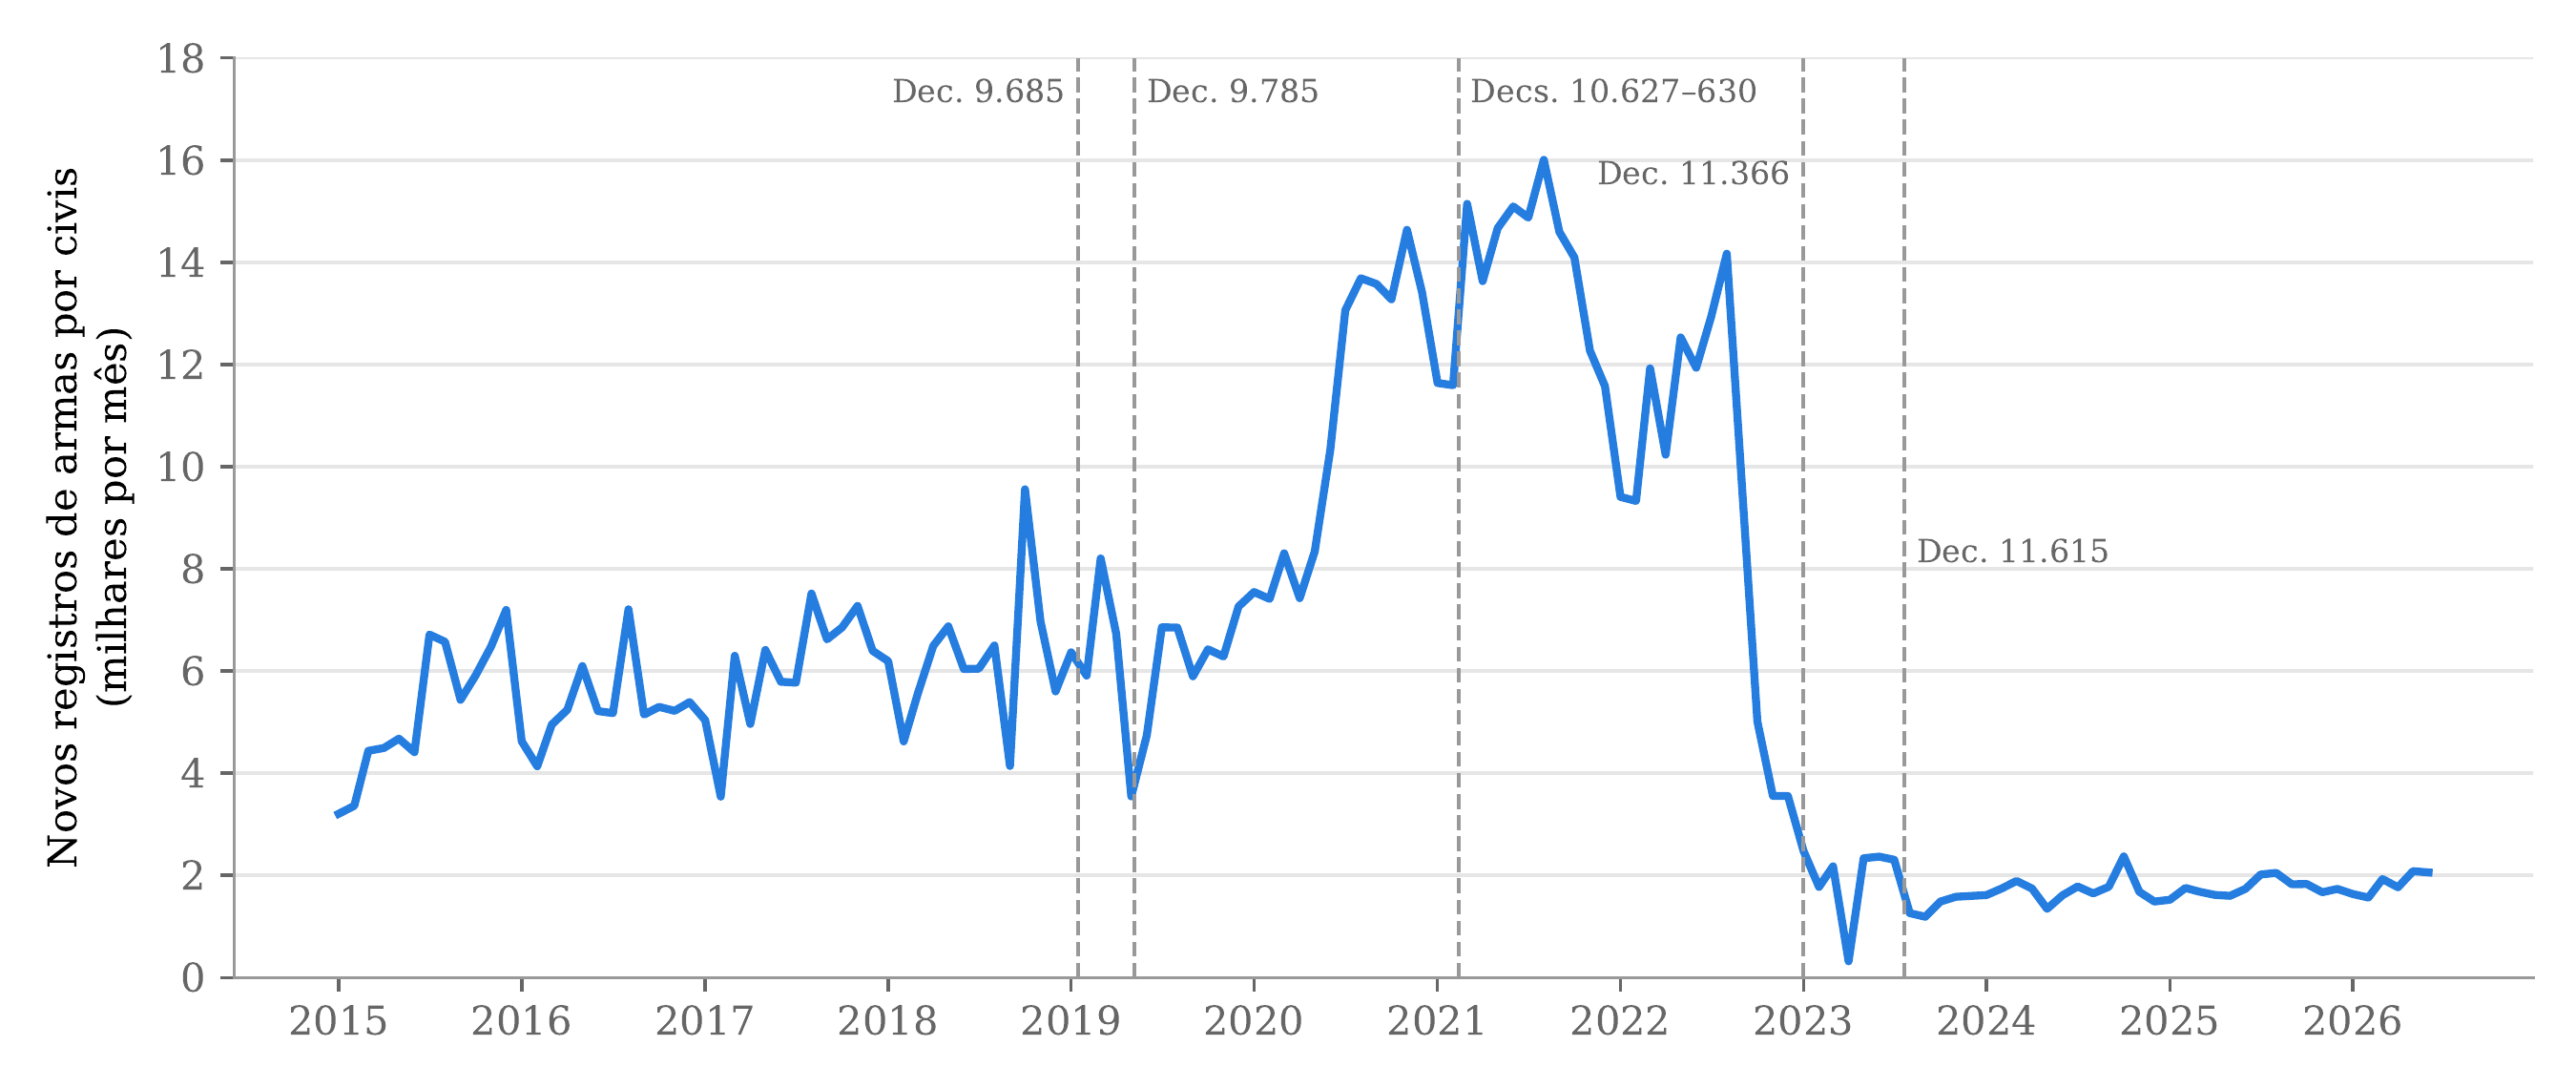
\includegraphics[width=\linewidth]{figs/registros_mensais_pt.png}
\caption{Figura 1 -- Novos registros mensais de armas de fogo por civis no Brasil e marcos regulatórios (2015--2026)}
\end{figure}

\nota{Fonte: elaborado pelos autores com base nos dados do SINARM/Polícia Federal.}

\subsection{Estratégia empírica}

Como os decretos alcançaram todo o território nacional ao mesmo tempo, a identificação explora a variação entre municípios na intensidade com que o choque se materializou:
\begin{equation}
Y_{it} = \alpha_i + \lambda_t + \beta\,(\Delta REG_i \times Pos_t) + X_{it}'\gamma + \varepsilon_{it},
\end{equation}
em que $Y_{it}$ é a taxa de homicídios por arma de fogo por 100 mil habitantes, $\alpha_i$ e $\lambda_t$ são efeitos fixos de município e de ano, $Pos_t$ indica os anos a partir de 2019 e $X_{it}$ reúne os controles. As regressões são ponderadas pela população, com erros-padrão agrupados por município. Estima-se também um modelo de Poisson com efeitos fixos para as contagens de óbitos e versões com as interações $\Delta REG_i \times Pos_t \times Fronteira_i$ e $\Delta REG_i \times Pos2023_t$.

Como o estimador de efeitos fixos bidirecionais pode ser viesado quando o momento do tratamento varia e os efeitos são heterogêneos \citep{goodmanbacon2021,roth2023}, utiliza-se o estimador de \citet{callaway2021}, com coortes definidas pelo primeiro ano entre 2019 e 2021 em que a taxa de registros do município atingiu o dobro de sua média de 2015--2018. A tripla diferença compara homicídios por arma de fogo e por arma branca no mesmo município e ano, absorvendo choques locais que afetem a violência em geral, e o \textit{synthetic difference-in-differences} \citep{arkhangelsky2021} reconstrói a trajetória pré-tratamento dos municípios tratados com pesos de unidades e de tempo. Na fronteira da soja, esses estimadores comparam os municípios de expansão recente com os produtores consolidados e com os municípios sem soja.

\section{Resultados e discussão}

\subsection{Efeito da expansão dos registros sobre os homicídios}

A Tabela 1 apresenta os resultados principais. Na especificação com controles, cada novo registro por mil habitantes eleva a taxa de homicídios por arma de fogo em @@b2@@ óbitos por 100 mil (erro-padrão de @@b2se@@), o que equivale a @@iqr@@ óbitos por 100 mil entre o primeiro e o terceiro quartil de exposição, ou @@pctiqr@@\% da taxa média. O modelo de Poisson indica aumento de @@pois@@\% por registro adicional por mil habitantes. A interação com a fronteira agrícola não é significativa (@@fint@@; p = @@fintp@@), e o termo de 2023 não indica reversão até 2024. O estimador de \citet{callaway2021} indica @@cs@@ óbitos adicionais por 100 mil nos municípios que experimentaram um salto de registros (erro-padrão de @@csse@@).

\noindent\textit{Tabela 1 -- Efeito da expansão dos registros de armas sobre os homicídios por arma de fogo}

TABELA@tab2@

\nota{Nota: variável dependente igual aos homicídios por arma de fogo por 100 mil habitantes; na coluna (5), contagem de óbitos com \textit{offset} igual ao logaritmo da população. A coluna (6) apresenta o ATT do estimador de Callaway e Sant'Anna. Erros-padrão agrupados por município entre parênteses. * p<0,10; ** p<0,05; *** p<0,01. Fonte: elaborado pelos autores.}

A Figura 2 apresenta a dinâmica do efeito. Os coeficientes posteriores a 2019 são positivos e significativos em todos os anos e atingem o maior valor em 2022--2023, período de maior estoque acumulado. Os coeficientes de 2015 a 2017 também são positivos, e o teste conjunto rejeita sua nulidade (p = @@wp@@), o que reflete em parte a queda acentuada dos homicídios em 2018 nos municípios de maior exposição. No estimador de \citet{callaway2021}, que compara cada coorte com seus próprios anos anteriores, os coeficientes pré-tratamento não são significativos e os efeitos posteriores são positivos e crescentes.

\begin{figure}
\centering
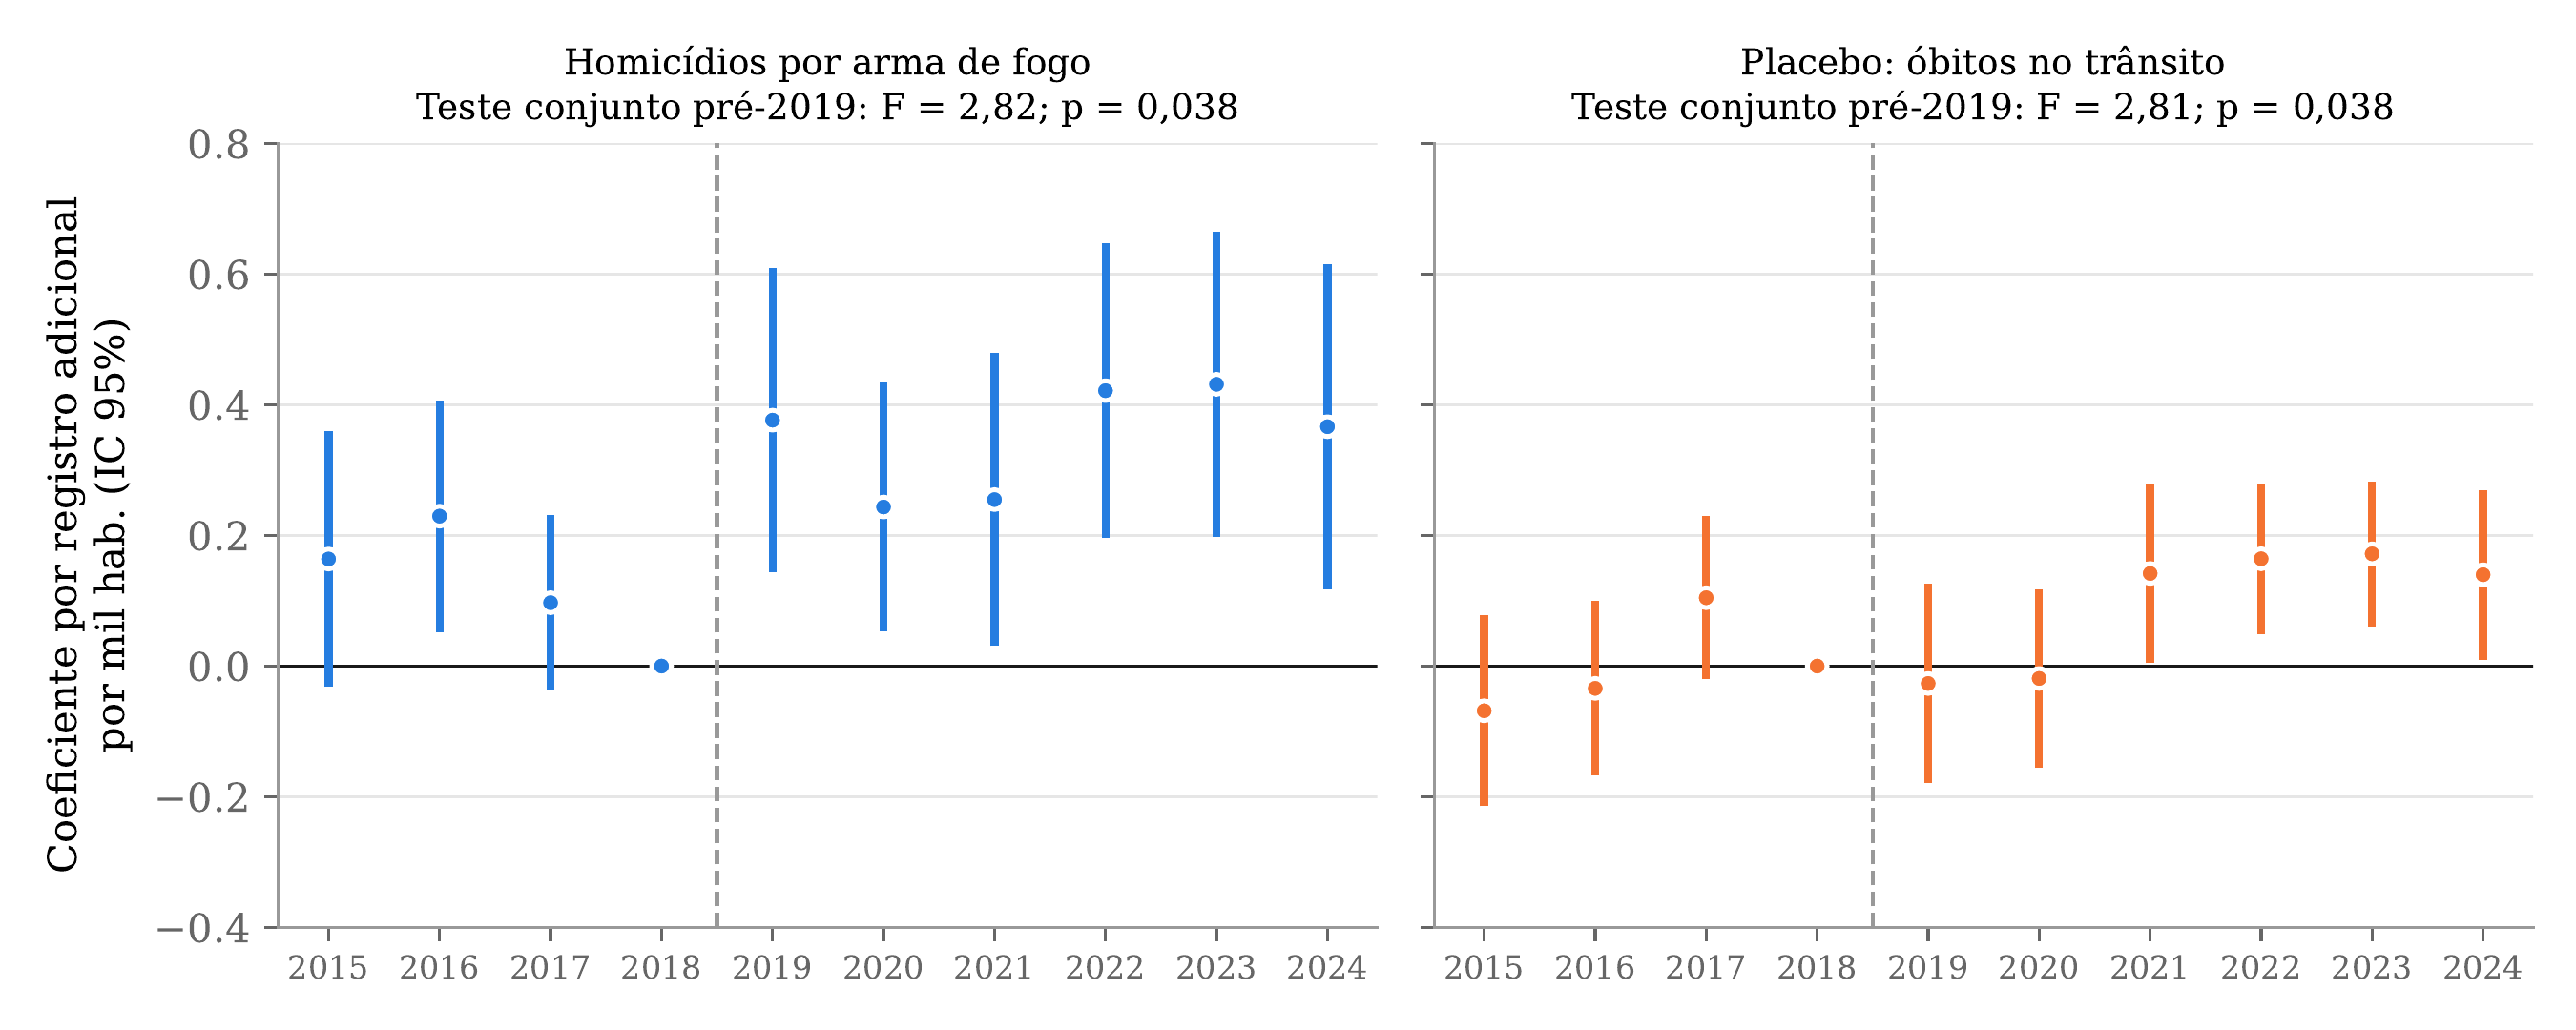
\includegraphics[width=\linewidth]{figs/event_study_pt.png}
\caption{Figura 2 -- Estimativas dinâmicas do efeito da expansão dos registros (ano de referência: 2018)}
\end{figure}

\nota{Nota: coeficientes por registro adicional por mil habitantes, com intervalos de confiança de 95\%. Fonte: elaborado pelos autores.}

\subsection{Robustez}

A Tabela 2 reúne os testes de robustez. A tripla diferença é positiva e significativa (@@ddd@@; p = @@dddp@@), e os homicídios por arma branca não respondem à expansão dos registros (@@ab@@; p = @@abp@@): o aumento da letalidade é específico ao meio arma de fogo, coerente com o canal de disponibilidade. Controles mais exigentes, com tendências por nível de registros anterior a 2019 ou efeitos fixos de UF por ano, elevam o coeficiente para cerca de @@ufano@@. Dois resultados recomendam cautela: o placebo com óbitos no trânsito é positivo no modelo de efeitos fixos (@@tr@@; p = @@trp@@), embora não no estimador de \citet{callaway2021} (@@cstr@@; erro-padrão de @@cstrse@@), e o placebo temporal de 2017 é marginalmente significativo. O \textit{synthetic difference-in-differences} confirma o efeito na comparação entre a coorte de 2019 e os municípios nunca tratados (@@c2@@; erro-padrão de @@c2se@@), mas não na comparação entre os quartis extremos de exposição (@@sdb@@; erro-padrão de @@sdbse@@), cujos municípios pertencem a regiões com dinâmicas de violência distintas.

\noindent\textit{Tabela 2 -- Testes de robustez}

TABELA@tab4@

\nota{Nota: todas as regressões incluem efeitos fixos de unidade e de tempo; salvo indicação, controles e ponderação pela população como na coluna (2) da Tabela 1. Erros-padrão agrupados por município. * p<0,10; ** p<0,05; *** p<0,01. Fonte: elaborado pelos autores.}

\subsection{A fronteira da soja}

A Tabela 3 mostra que a fronteira da soja recebeu mais armas após 2019 do que os produtores consolidados e os municípios sem soja. Contra os municípios sem soja, a diferença em diferenças indica @@soydid@@ homicídios adicionais por 100 mil, mas os coeficientes anteriores a 2019 sugerem uma trajetória de alta já em curso, compatível com a interiorização da violência (p do teste conjunto igual a @@soyesp@@). Os estimadores que lidam com essa trajetória confirmam o efeito. O \textit{synthetic difference-in-differences} contra os produtores consolidados, que compara municípios com a mesma base produtiva, estima @@soysd@@ óbitos por 100 mil (erro-padrão de @@soysdse@@). Na versão escalonada do estimador de \citet{callaway2021}, em que cada município da fronteira entra no tratamento no ano de seu primeiro salto de registros, o efeito é de @@soycs@@ óbitos por 100 mil (erro-padrão de @@soycsse@@; p = @@soycsp@@), sem coeficientes pré-tratamento significativos. O efeito na fronteira da soja é, portanto, cerca de @@soyratio@@ vezes a média nacional, concentrado em municípios pequenos e médios, já que deixa de ser significativo quando os municípios tratados são ponderados pela população.

\noindent\textit{Tabela 3 -- A fronteira da soja como grupo tratado}

TABELA@tab6@

\nota{Nota: fronteira da soja definida por municípios da Amazônia e do Cerrado com ao menos 1.000 ha de soja em 2018, área de soja 50\% maior que em 2010 e perda de vegetação primária entre 2015 e 2018 acima da mediana do bioma. No estimador escalonado de Callaway e Sant'Anna, as coortes são definidas pelo primeiro salto de registros. * p<0,10; ** p<0,05; *** p<0,01. Fonte: elaborado pelos autores com base em IBGE, MapBiomas, SINARM e SIM.}

\subsection{Desmatamento e armas}

A Tabela 4 examina a associação entre desmatamento e registros de armas. Dentro do mesmo município, os anos de maior desmatamento são acompanhados de mais registros, mesmo com efeitos fixos de UF por ano (@@dp1@@; p = @@dp1p@@), e a associação persiste com o desmatamento do ano anterior (@@dplag@@; p = @@dplagp@@). Entre municípios, o desmatamento de 2015--2018 prevê a expansão de registros em 2019--2022 no Cerrado (@@dbce@@; p = @@dbcep@@), mas não na Amazônia nem no país como um todo. No tercil de maior desmatamento, os novos registros cresceram @@t3pct@@\% após 2019, enquanto ficaram estáveis no tercil de menor desmatamento. Essas associações não têm interpretação causal, pois desmatamento e demanda por armas podem resultar de um mesmo processo de expansão agropecuária e de disputa por terra, mas indicam que, no Cerrado, desmatamento, armas e homicídios caminham juntos.

\noindent\textit{Tabela 4 -- Desmatamento e registros de armas por civis}

TABELA@tab7@

\nota{Nota: no Painel A, variável dependente igual aos novos registros por mil habitantes no ano, com efeitos fixos de município e ponderação pela população; no Painel B, novos registros de 2019--2022 por mil habitantes contra o desmatamento acumulado em 2015--2018, com controles e efeitos fixos de UF. * p<0,10; ** p<0,05; *** p<0,01. Fonte: elaborado pelos autores com base em MapBiomas, SINARM e IBGE.}

\subsection{Discussão}

Os resultados alinham-se às evidências de \citet{duggan2001}, \citet{cook2006} e \citet{cerqueira2012}: a ampliação do estoque de armas legais elevou os homicídios por arma de fogo pelo canal de disponibilidade, sem dissuasão visível nas demais formas de homicídio. A magnitude é moderada no país como um todo e ocorreu durante a queda nacional dos homicídios, que a flexibilização não reverteu, mas atenuou nos municípios mais expostos. Nos territórios de expansão da soja, porém, o efeito é cerca de duas vezes maior, o que indica que a política federal de armas interagiu com as dinâmicas fundiárias e produtivas da fronteira agrícola.

A análise tem limitações. A medida de tratamento cobre as armas de posse de civis e não inclui os caçadores, atiradores e colecionadores, cujos registros não são divulgados por município. Os testes pré-tratamento do \textit{event study} convencional e o placebo com óbitos no trânsito sugerem que parte da associação pode refletir choques locais concomitantes, preocupação atenuada, mas não eliminada, pelos estimadores robustos. A causalidade reversa não pode ser descartada, e o desenho da fronteira da soja não separa inteiramente a flexibilização das armas de outros choques do agronegócio no período, como a alta dos preços das \textit{commodities}.

\section{Conclusões}

A flexibilização do acesso a armas de fogo entre 2019 e 2022 elevou os homicídios por arma de fogo nos municípios brasileiros mais expostos ao choque, com efeito especialmente intenso na fronteira da soja do Cerrado e da Amazônia. Cada novo registro de arma por mil habitantes aumentou a taxa de homicídios por arma de fogo em cerca de @@b2@@ óbitos por 100 mil ao ano, e os municípios da fronteira da soja que experimentaram um salto de registros tiveram, em média, @@soycs@@ óbitos adicionais por 100 mil. O efeito é específico às mortes por arma de fogo e persistiu após a restrição de 2023, compatível com a permanência do estoque acumulado.

Para a governança dos territórios rurais, os resultados indicam que a expansão agropecuária recente combina pressão sobre a vegetação nativa, aumento das armas em circulação e violência letal. Políticas de segurança pública para o campo devem considerar o estoque de armas acumulado entre 2019 e 2022, priorizar a fiscalização nos municípios de fronteira agrícola e integrar as bases de registros de armas, de mortalidade e de monitoramento territorial. A divulgação dos registros de caçadores, atiradores e colecionadores por município permitiria avaliações mais completas.

\bibliographystyle{plainnat}
\bibliography{referencias}

\end{document}
